\documentclass[aspectratio=169,usenames,dvipsnames]{beamer}
\usepackage{../packages_beamer}
\usetheme{Madrid}
\usecolortheme{beaver}

\usepackage{tikz}
\newcommand{\xdownarrow}[1]{%
  {\left\downarrow\vbox to #1{}\right.\kern-\nulldelimiterspace}
}
\usepackage[export]{adjustbox}
\usepackage{wrapfig}
\usepackage{caption}
\usepackage{pifont}
\usepackage{smartdiagram}
\usepackage{tcolorbox}
\tcbuselibrary{theorems}
\usepackage{amsmath}
\usepackage{unicode-math}
\usepackage[absolute,overlay]{textpos}
\usepackage{multimedia}

\newcommand*{\colorboxed}{}
\def\colorboxed#1#{%
  \colorboxedAux{#1}%
}
\newcommand*{\colorboxedAux}[3]{%
  % #1: optional argument for color model
  % #2: color specification
  % #3: formula
  \begingroup
    \colorlet{cb@saved}{.}%
    \color#1{#2}%
    \boxed{%
      \color{cb@saved}%
      #3%
    }%
  \endgroup
}

\newcommand{\filt}[1]{\overline{#1}^\ell}

\def\boxit#1{%
  \smash{\color{red}\fboxrule=1pt\relax\fboxsep=2pt\relax%
  \llap{\rlap{\fbox{\vphantom{0}\makebox[#1]{}}}~}}\ignorespaces
}

\captionsetup[figure]{labelformat=empty}
\beamertemplatenavigationsymbolsempty
\title[Stage L3 Physique - Paris-Saclay/LISN]{Analyse statistique d'un écoulement turbulent}
\subtitle{}
\author[Nikita Allaglo]{Nikita Allaglo \\
Soutenance orale de mon stage du 2 mai au 4 juillet sous la supervision de Caroline Nore}
\date[03-07-2023]{3 juillet 2023}

\AtBeginSection[]
{
    \begin{frame}
        \frametitle{Plan de la présentation}
        \tableofcontents[currentsection]
    \end{frame}
}

\begin{document}

%title

\begin{frame}
\titlepage
\begin{figure}
    \centering
    
\includegraphics[width=0.2\textwidth]{figs/logo_PS.jpg} 
    
\includegraphics[width=0.2\textwidth]{figs/logo_lisn.png}
\end{figure}
\end{frame}

% feynman quote, institut clay price, french washing machine
\begin{frame}{Motivation}{Recherche fondamentale}
\begin{columns}
    \column{.2\textwidth}
    \begin{figure}
        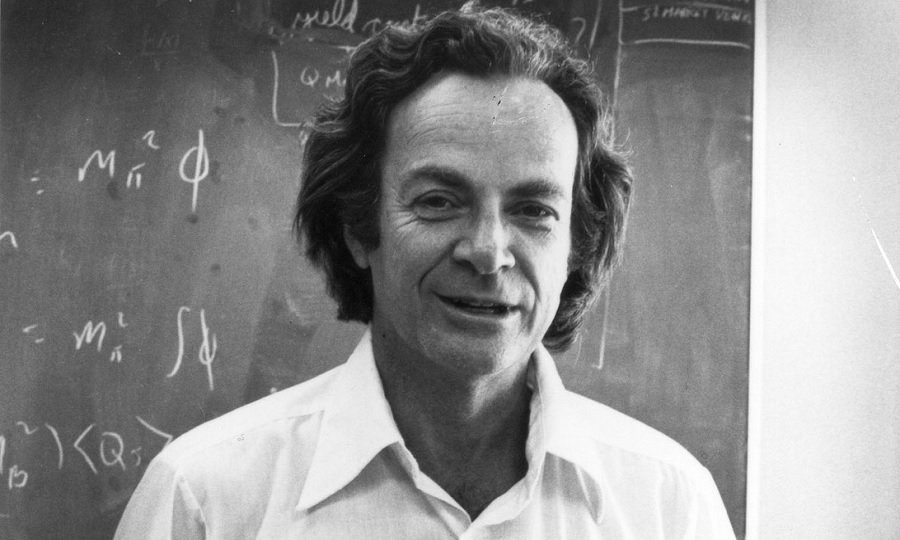
\includegraphics[width=.95\linewidth, center]{figs/feynman.jpg}
    \end{figure}\hfill
    \column{.8\textwidth}
    \begin{block}{Richard Feynman (1964)}
        \textit{La turbulence est le problème non résolu le plus important de la physique classique.}
    \end{block}
\end{columns}\pause
\centering
{\bf Problèmes du prix du millénaire}
\begin{figure}
    
\includegraphics[height=.1\textheight, center]{figs/clay.jpeg}
\end{figure}\pause
\begin{tcolorbox}[colback=Goldenrod!5!white,colframe=Goldenrod]
    Pour 3 dimensions spatiales et une temporelle, étant donné un champ de vitesse initial, 
    existe-il un champ de vitesse ainsi qu'un champ scalaire de pression 
    \colorboxed{red}{\text{partout continus et définis}} qui résolvent les équations de Navier-Stokes ?
\end{tcolorbox}
\end{frame}

\begin{frame}{Motivation}{Aspects statistiques (Figures tirées de {\color{blue}U. Frisch, \emph{Turbulence: The Legacy of A. N. Kolmogorov} (1995)})}
    \begin{figure}
        \centering
        \onslide<1->{\begin{subfigure}[b]{0.42\textwidth}
            \centering
        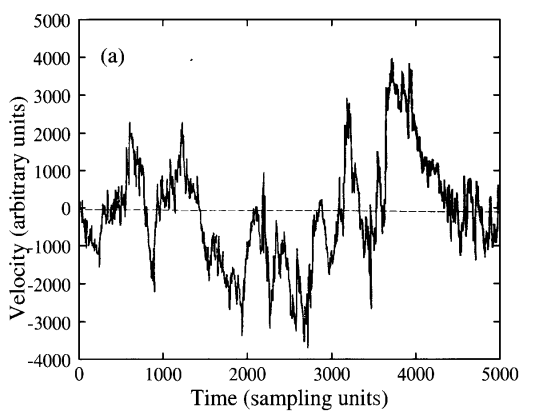
\includegraphics[height=0.4\textheight, width=\linewidth]{figs/frisch_t1.png}
        \end{subfigure}}
        \onslide<3->{\begin{subfigure}[b]{0.42\textwidth}
            \centering
        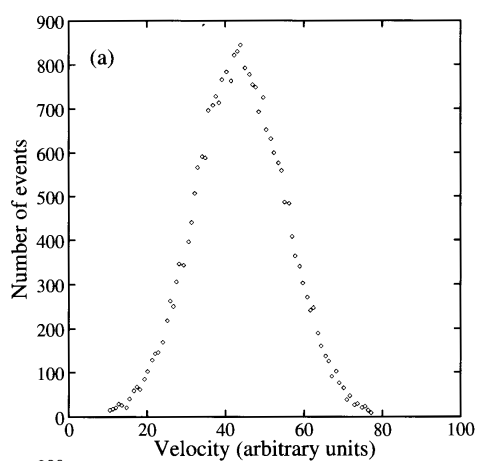
\includegraphics[height=0.4\textheight, width=\linewidth]{figs/frisch_stat1.png}
        \end{subfigure}}
        \onslide<2->{\begin{subfigure}[b]{0.42\textwidth}
            \centering
        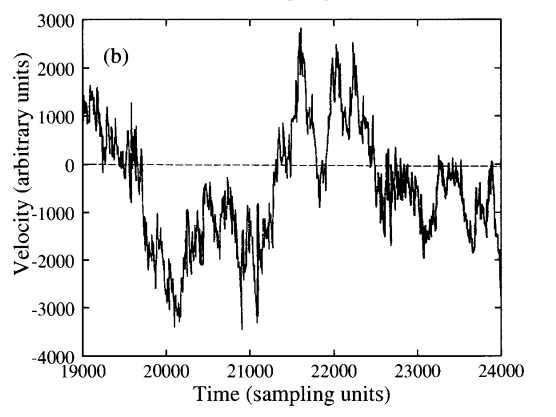
\includegraphics[height=0.4\textheight, width=\linewidth]{figs/frisch_t2.png}
        \end{subfigure}}
        \onslide<3->{\begin{subfigure}[b]{0.42\textwidth}
            \centering
        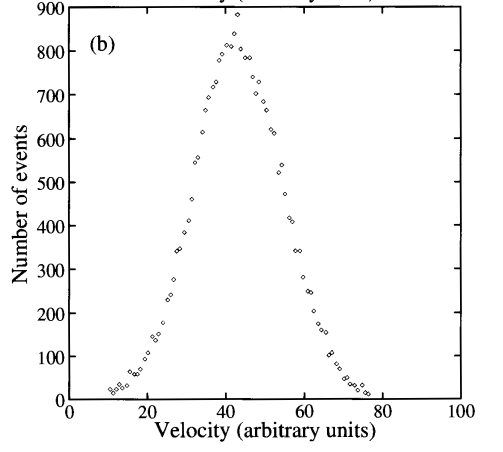
\includegraphics[height=0.4\textheight, width=\linewidth]{figs/frisch_stat2.png}
        \end{subfigure}}
    \end{figure}
\end{frame} % add arrows between the plots + séquentialiser les apparitions

\begin{frame}
    \frametitle{Plan de la présentation}
    \tableofcontents
\end{frame}

\section{La turbulence hydrodynamique}

\subsection{Nombre de Reynolds}
\begin{frame}{Nombre de Reynolds}
    \begin{tcolorbox}[title={Équation de Navier-Stokes adimensionnée},
        colback=Goldenrod!5!white,colframe=Goldenrod, coltitle=black]
        \begin{gather}
        \del_t \git{u} + \only<1-3>{\qty(\git{u}\cdot\grad)\git{u}} 
        \only<4->{\colorboxed{red}{\qty(\git{u}\cdot\grad)\git{u}}} = -\grad p + 
        \dfrac{1}{\text{Re}}\only<1>{\grad^2\git{u}} 
        \only<2->{\colorboxed{blue}{\grad^2\git{u}}} + \frac{L}{U^2}\git{f},\\
        \text{Re} = \dfrac{UL}{\nu},
       \end{gather}
    \end{tcolorbox}
    avec $\git{u}$ la vitesse, $p$ la pression (adimensionnées), $\git{f}$ les forces externes
    par densité massique; $\nu$ étant la viscosité du fluide et $U,L$ la vitesse et la longueur caractéristiques de l'écoulement.
    \begin{itemize}[label=\ding{43}]
        \item \onslide<3->{{\color{blue}$\text{Re}\ll 1$: domination de la dissipation visqueuse}}
        \item \onslide<5->{{\color{red}$\text{Re}\gg 1$: domination de la convection ({\bf non-linéarités})}}
    \end{itemize}
\end{frame} % séquentialiser les apparitions 

\subsection{Dissipation anormale}
\begin{frame}{Dissipation anormale}
    \begin{tcolorbox}[colback=Goldenrod!5!white,colframe=Goldenrod, coltitle=black,
        title={Zéroième loi de la turbulence}]
		La puissance injectée moyenne (ou le taux moyen de variation de l'énergie cinétique) au sein 
    d'un fluide tend vers une constante non-nulle à viscosité rigoureusement nulle.
\end{tcolorbox}\pause
\begin{columns}
\column{0.6\textwidth}
\begin{figure}[h]
    \centering
    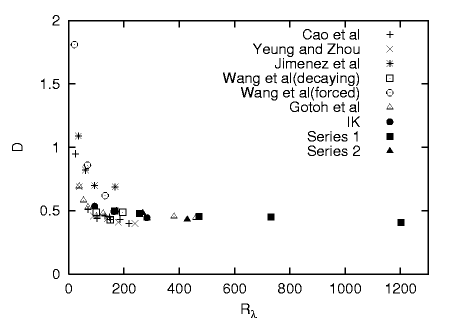
\includegraphics[height=0.45\textheight, width=0.8\linewidth]{figs/anomalous.png}
    \caption{Figure tirée de {\color{blue}Kaneda \emph{et al.}, Physics of Fluids {\bf 15}, 2 (2003)}}
  \end{figure}
\column{0.4\textwidth}\pause
\centering
\onslide<5->{\bf Conjecture d'Onsager (1949)}
\begin{gather}
    \onslide<3->{\qty(\omega = |\grad\wedge\git{u}|)\\
    \pdv{\mean{E}}{t} = \rho\nu\mean{\omega^2}\\}
    \onslide<4->{\underset{\nu\to 0}{\to}C\\}
    \onslide<5->{\Downarrow\nonumber\\}
    \onslide<5->{\colorboxed{red}{\mean{\omega^2}\underset{\nu\to 0}{\to}\infty~?}}
\end{gather}
\end{columns}
\end{frame}

% \subsection{Théorie de Kolmogorov}
% \begin{frame}{Lois de Kolmogorov}
% \end{frame}

\subsection{Formulation faible}
\begin{frame}{Formulation faible}{K41}
\centering
\begin{columns}
    \column{.8\textwidth}
    \begin{block}{Théorie de Kolmogorov (1941)}
        \begin{itemize}[label=\ding{43}]
            \item Existence d'une zone inertielle $\eta\ll \ell\ll L$ permettant les cascades énergétiques
                  ($\eta$ échelle de Kolmogorov, $L$ échelle d'injection d'énergie)
            \item Captage des échelles à l'aide d'\ul{incr\'ements} $\delta u_\ell(\git{x})=\base{\ell}
                  \cdot\qty(\git{u}(\git{x}+\git{\ell})-\git{u}(\git{\ell}))$
            \item Lois universelles autour de {\bf fonctions de structure} $S_p(\ell):=\mean{|\delta u_\ell|^p}$
            \item Défauts: le cadre mathématique ne donne pas de sens aux singularités, 
                  turbulence statistiquement homogène et isotrope ...
        \end{itemize}
    \end{block}\hfill
    \column{.2\textwidth}
    \begin{figure}
        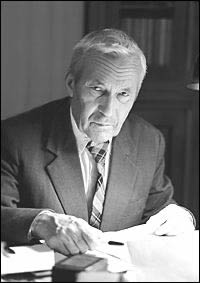
\includegraphics[height=.4\textheight, center]{figs/Andrej-Kolmogorov_595e00fb51178.jpg}
    \end{figure}
\end{columns}
\end{frame} % séquentialiser les apparitions

\begin{frame}{Formulation faible}{Incorporer les singularités}
\centering
{\bf Comment prendre en compte de potentielles singularités ?}\pause\\
Théorie des distributions\pause\\
Espace de fonctions tests: $\varphi>0\in\mathscr{C}^
\infty$ à support compact dans $\mathbb{R}^3$ et s'intégrant à l'unité.\pause
\vspace{0.2cm}
\begin{columns}
    \column{0.4\textwidth}
    \centering
    Lissage:
    \begin{gather}
        \varphi_\ell(\git{\xi}) := \dfrac{1}{\ell^3}\varphi\qty(\dfrac{\git{\xi}}{\ell})\nonumber\\
        \filt{X}(\git{r}) = \mathlarger{\int_{\mathbb{R}^3}}\varphi_\ell(\git{\xi})
    X(\git{\xi}+\git{r})\dd^3\git{\xi}\nonumber
    \end{gather}\pause
    \column{0.6\textwidth}
    \centering
    Énergie pseudo-filtrée: $\tilde{E}_\ell:=\rho\frac{\git{u}\cdot\filt{\git{u}}}{2}$
    \begin{align}
        \colorboxed{red}{\del_t \tilde{E}_\ell + \div{\git{J}^{\text{NS}}_\ell} + 
        \mathscr{D}^\nu_\ell + \mathscr{D}^{u}_\ell
        = \mathcal{P}_\ell}
    \end{align}\pause
    \begin{tcolorbox}[colback=Goldenrod!5!white,colframe=Goldenrod, coltitle=black,
        title={Dissipation anormale}]
		\begin{equation}
            \mathscr{D}^{u}_\ell =   \frac{\rho}{2} (\git{u}\cdot  \filt{u_i  \del_i \git{u}}
     -  u_i\git{u}\cdot \del_i \filt{\git{u}})
        \end{equation}
\end{tcolorbox}
\end{columns}
\end{frame}

\section{Problématique du stage}
\subsection{Géométrie de l'écoulement de von-Karman et simulations numériques}
\begin{frame}{Géométrie de l'écoulement de von-Karman et simulations numériques}
\begin{columns}
\column{0.6\textwidth}
\begin{figure}[h]
    \centering
    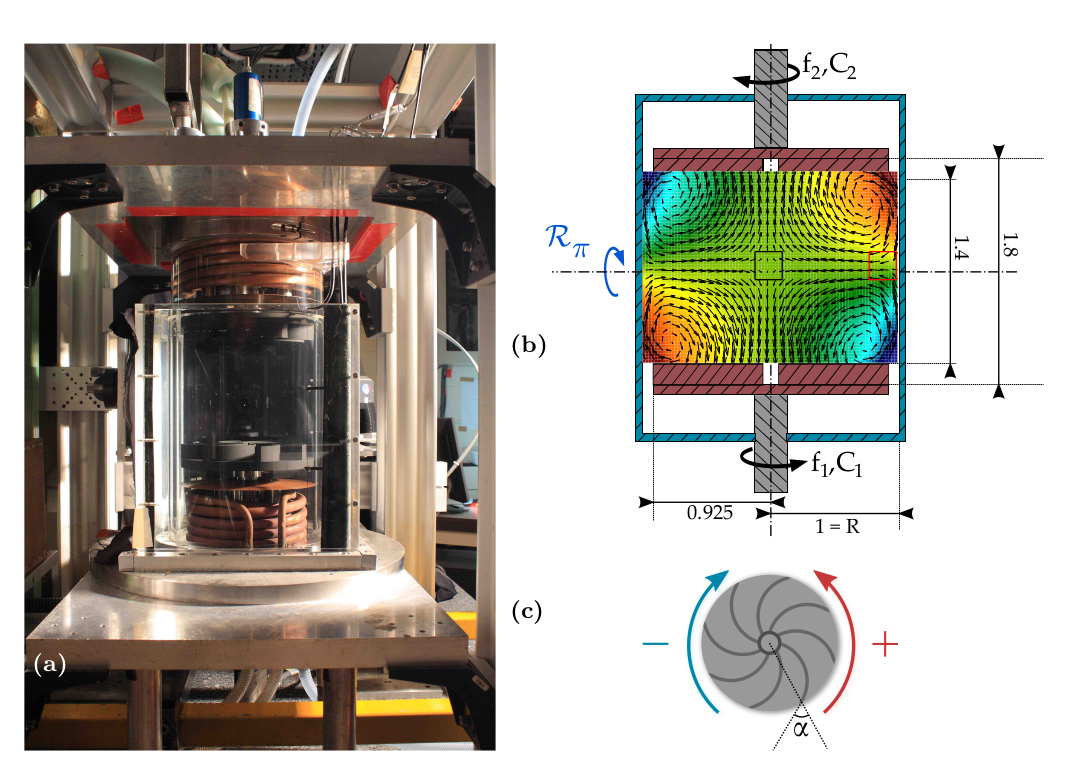
\includegraphics[height=0.7\textwidth]{figs/geometrie_vk.png}
    \caption{Figure tirée de {\color{blue}Dubrulle, JFM {\bf 867}, 1 (2019)}}
\end{figure}\pause
\column{0.4\textwidth}
\centering Simulations numériques SFEMaNS\pause: 
\begin{itemize}[label=\ding{43}]
    \item {\small Résout Navier-Stokes $(\git{u})$ et permet de calculer toutes les grandeurs
          d'intérêt dans l'écoulement (dissipations, vorticité, filtrages)}\pause
    \item {\small code hautement parallèle (Fast Fourier Transform pour coordonnées angulaires, 
          éléments finis pour $(r,z)$)}\pause
    \item {\small forte résolution {\bf spatiale} mais limitations pour Re et snapshots}
\end{itemize}
\end{columns}
\end{frame}

\subsection{Faller \emph{et al.}, Journal of Fluid Mechanics {\bf 914}, 2 (2021)}
\begin{frame}{Faller \emph{et al.}, Journal of Fluid Mechanics {\bf 914}, 2 (2021)}
    \begin{table}%[ht]
        \begin{center}
        \def~{\hphantom{0}}
        \begin{tabular}
        {|llcrrlllc|}%
        %\hline \hline
         Cas &F (\SI{}{\hertz})& Points de grille &$\text{Re}\quad $ &$\epsilon (\text{adim})$ &$\eta$(\SI{}{\milli\metre})& 
        $\Delta x$(\SI{}{\milli\metre})\\[3pt]
        %\hline \hline
        %\hline
         A &$5$&$89 \times 65$&$3.1~10^5$&$0.045$& $0.016$&$2.1$\\
        %\hline
        B&$5$&$77 \times 79$&$3.1~10^5$&$0.045$&$0.016$&$0.49$\\
        %\hline
        C&$5$&$162\times157$&$3.1~10^5$&$0.045$&$0.016$&$0.24$\\
        %\hline
        D&$1$&$77 \times 80$&$4.1~10^4$&$0.045$&$0.073$&$0.49$\\
        %\hline
        E&$1.2$&$151\times174$&$5.8~10^3$&$0.045$&$0.32$&$0.24$\\
        %\hline
        T-$1$ &$5$&$149\times103\times20$&$3.1~10^5$&$0.045$&$0.016$&$0.35$\\%TPIV Paul
        %\hline
        T-$2$ &$1$&$139\times101\times20$&$6.3~10^4$&$0.045$&$0.054$&$0.35$\\%TPIV Paul
        %\hline
        T-$3$ &$0.5$&$148\times103\times20$&$3.1~10^4$&$0.045$&$0.09$&$0.35$\\%TPIV Paul
        %\hline
        T-$4$ &$0.1$&$149\times100\times20$&$6.3~10^3$&$0.045$&$0.3$&$0.35$\\%TPIV Paul
        %\hline
        \boxit{4.5in} DNS &$\frac{1}{2\pi}$&$400\times800\times509$&$6~10^3$&$0.045$&$0.37$&$0.1$-$0.4$\\%Hugues
        \end{tabular}
        \caption*{Paramètres décrivant les données utilisées dans 
        {\color{blue}Faller \emph{et al.}, JFM {\bf 914}, 2 (2021)}.
        $F$ est la fréquence de rotation des turbines;
        $Re$ est le nombre de Reynolds;
        $\epsilon$ est la dissipation énergétique totale adimensionnée ; $\eta$ est 
        l'échelle de Kolmogorov ;
        et $\Delta x$ représente la résolution spatiale dans les expériences 
        (dénotées de A à T-4) et les simulations numériques directes (dénotées DNS).}
        \label{tab:params_vk}
         \end{center}
        \end{table}%}
\end{frame}

\begin{frame}{Faller \emph{et al.}, Journal of Fluid Mechanics {\bf 914}, 2 (2021)}
    Faller effectue en premier lieu une analyse statistique primaire de l' écoulement de von-Karman:
    \begin{itemize}[label=\ding{43}]
        \item il considère les événements simultanés de $\mathscr{D}^I_\ell=
        \dfrac{\rho}{2}\grad\cdot\qty(\git{u}\filt{u^2}-\filt{u^2\git{u}}) 
        + \mathscr{D}^u_\ell$ et $\omega=|\grad\wedge \git{u}|$\pause
        \item pour les échelles de filtrage $\ell=1.06\eta$ et $\ell=26.5\eta$,
             il obtient un étrange jet de corrélations\pause
        \item Questionnements effectués par les auteurs:
            \begin{columns}
            \column{0.5\textwidth}
            \begin{figure}[h]
                \centering
                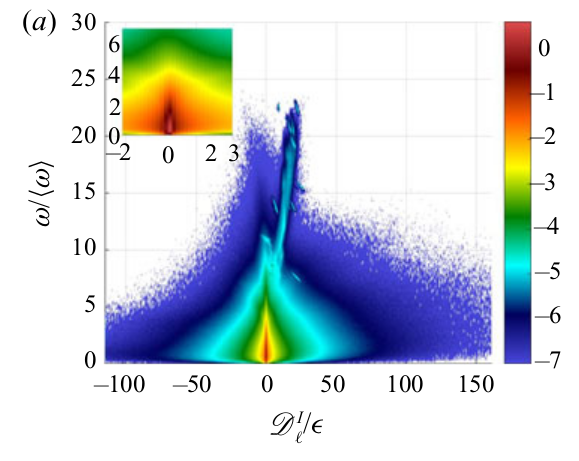
\includegraphics[width=\linewidth, height=0.6\textheight]{figs/faller_l1_dns_2.png}
            \end{figure}\pause
            \column{0.5\textwidth}
              \begin{itemize}[label=\ding{112}]
                \item $\grad\cdot\git{u} \neq 0$ ?\pause
                \item $\filt{\git{u}}\underset{\ell\to 0}{\cancel\to} \git{u}$ sur l'axe ?\pause
                \item $\mathscr{D}^I_\ell$ vs $\mathscr{D}^u_\ell$ ?\pause
                \item conditions aux limites strictes vs ouvertes ?
              \end{itemize}
            \end{columns}
    \end{itemize}
\end{frame}

\subsection{Tâches assignées}
\begin{frame}{Tâches assignées}
\centering
{\bf L'équipe dispose d'une nouvelle base de données SFEMaNS (1.1 TB) répliquant les calculs
de Faller avec les correctifs.}\\
\vspace{.5cm}\pause
Mes réalisations ont principalement été les suivantes:\pause
\begin{itemize}[label=\ding{51}]
    \item développer un module d'analyse statistique permettant de calculer les grandeurs
          d'intérêt en turbulence (moyennes, moments, probabilités, probabilités conditionnelles, corrélations)\pause
    \item pouvoir appliquer ce module sur des bases de données géantes\pause
    \item déterminer l'origine du jet de corrélations chez Faller\pause
\end{itemize}
\begin{columns}
    \column{0.7\textwidth}
    \begin{figure}[h]
        \centering
        
\includegraphics[width=\linewidth]{figs/module.png}
    \end{figure}
    \href{https://gitlab.lisn.upsaclay.fr/allaglo/von-karman-postprocess}
    {https://gitlab.lisn.upsaclay.fr/allaglo/von-karman-postprocess}
    \column{0.3\textwidth}
    \centering
    2 branches permettant d'optimiser CPUs/GPUs.
\end{columns}
\end{frame} % dire formellement ce que j'ai fait
% 

% \section{Méthodes}
% \subsection{Module d'analyse statistique}
% % généralités sur les stats, capable de compute tout, dispose d'une branche CPU et GPU
% % pour l'optimisation (expliciter les temps d'exécution pour des workloads typiques)
% % mentionner l'adresse du git et les tutoriels
% \begin{frame}{Module d'analyse statistique}
% \end{frame}

% \subsection{Gestion de la mémoire} % comment réellement post-process sur des 
% \begin{frame}{Module d'analyse statistique}
% \end{frame}

\section{Résultats}
\subsection{Comparaison des probabilités jointes numériques}
\begin{frame}{Comparaison des probabilités jointes numériques}{$\ell=1.06\eta$ 
    (GAUCHE: Allaglo; DROITE: Faller et al.)}
\begin{figure}[H]
    \centering
    \begin{subfigure}[b]{0.48\linewidth}
    \centering
    \includegraphics[width=\textwidth]{../rapport/figs/figs_rapport/joint_D001_DR_omega_penal.jpg}
    \end{subfigure}
    \begin{subfigure}[b]{0.4\linewidth}
      \centering
      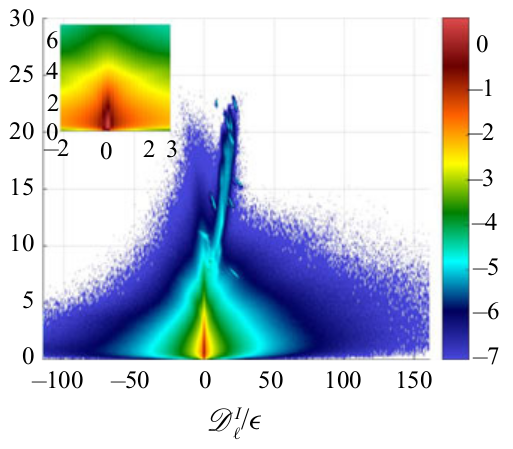
\includegraphics[width=\textwidth]{figs/faller_l1_dns.png}
      \end{subfigure}
    \label{fig:DR_penal}
  \end{figure}
\end{frame}

\begin{frame}{Comparaison des probabilités jointes numériques}{$\ell=26.5\eta$
    (GAUCHE: Allaglo; DROITE: Faller et al.)}
    \begin{figure}[H]
        \centering
        \begin{subfigure}[b]{0.48\linewidth}
        \centering
        \includegraphics[width=\textwidth]{../rapport/figs/figs_rapport/joint_D002_DR_omega_penal.jpg}
        \end{subfigure}
        \begin{subfigure}[b]{0.4\linewidth}
          \centering
          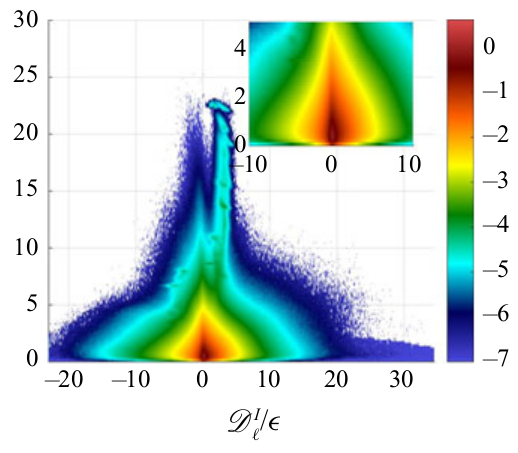
\includegraphics[width=\textwidth]{figs/faller_l2_dns.png}
          \end{subfigure}
        \label{fig:DR_penal}
      \end{figure}
    \begin{itemize}[label=\ding{51}]\pause
        \item Validation du module \texttt{von-Karman-PostProcess}\pause
        \item {\color{green}$\filt{\git{u}}\underset{\ell\to 0}{\cancel\to} \git{u}$ sur l'axe}
    \end{itemize}
    \end{frame}

\subsection{Comparaison des probabilités jointes numériques et expérimentales}

\begin{frame}{Comparaison des probabilités jointes numériques et expérimentales}{GAUCHE: Allaglo, $\ell=1.06\eta$; 
    DROITE: Faller et al., $\ell=3.2\eta$}
    \begin{figure}[H]
        \centering
        \begin{subfigure}[b]{0.48\linewidth}
        \centering
        \includegraphics[width=\textwidth]{../rapport/figs/figs_rapport/DDR1_omega_bulk.jpg}
        \end{subfigure}
        \begin{subfigure}[b]{0.4\linewidth}
          \centering
          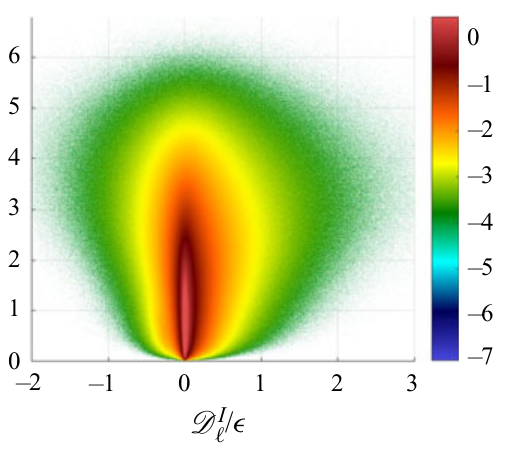
\includegraphics[width=\textwidth]{figs/faller_l1_exp.png}
          \end{subfigure}
        \label{fig:DR_penal}
      \end{figure}
    \end{frame}
    
    \begin{frame}{Comparaison des probabilités jointes numériques et expérimentales}{GAUCHE: Allaglo, $\ell=26.5\eta$; 
        DROITE: Faller et al., $\ell=17.9\eta$}
        \begin{figure}[H]
            \centering
            \begin{subfigure}[b]{0.48\linewidth}
            \centering
            \includegraphics[width=\textwidth]{../rapport/figs/figs_rapport/DDR2_omega_bulk.jpg}
            \end{subfigure}
            \begin{subfigure}[b]{0.4\linewidth}
              \centering
              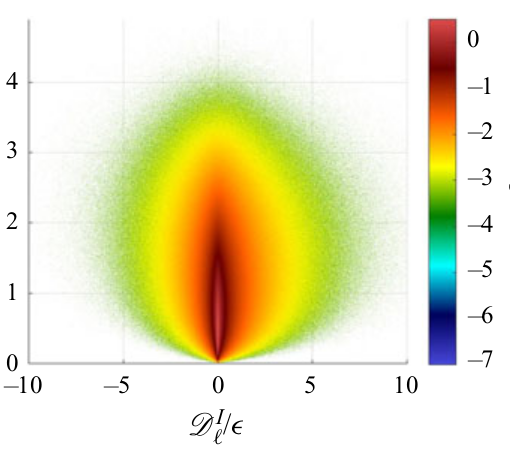
\includegraphics[width=\textwidth]{figs/faller_l2_exp.png}
              \end{subfigure}
            \label{fig:DR_penal}
          \end{figure}
          \begin{itemize}[label=\ding{51}]\pause
            \item Dissymétrie plus marquée à basses échelles pour num. et exp.\pause
            \item Cascade mieux mise en évidence numériquement
          \end{itemize}
        \end{frame}

\subsection{Comparaison entre $\mathscr{D}^u_\ell$ et $\mathscr{D}^I_\ell(=\mathscr{D}^{\mathrm{DR}}_\ell)$}
\begin{frame}{$\mathscr{D}^u_\ell$ vs $\mathscr{D}^I_\ell(=\mathscr{D}^{\mathrm{DR}}_\ell)$ (probabilités)}
\begin{figure}[H]
    \centering
    \begin{subfigure}[b]{0.48\linewidth}
    \centering
    \includegraphics[width=\textwidth]{../rapport/figs/figs_rapport/joint_D001_DR_Du_l1.jpg}
    \end{subfigure}
    \begin{subfigure}[b]{0.48\linewidth}
      \centering
      \includegraphics[width=\textwidth]{../rapport/figs/figs_rapport/joint_D002_DR_Du_2.jpg}
      \end{subfigure}
    \label{fig:dudr_joint}
  \end{figure}
\end{frame}

\begin{frame}{$\mathscr{D}^u_\ell$ vs $\mathscr{D}^I_\ell(=\mathscr{D}^{\mathrm{DR}}_\ell)$ (corrélations)}
    \begin{figure}[H]
        \centering
        \begin{subfigure}[b]{0.48\linewidth}
        \centering
        \includegraphics[width=\textwidth]{../rapport/figs/figs_rapport/corr_D001_DR_Du_l1.jpg}
        \end{subfigure}
        \begin{subfigure}[b]{0.48\linewidth}
          \centering
          \includegraphics[width=\textwidth]{../rapport/figs/figs_rapport/corr_D002_DR_Du_2.jpg}
          \end{subfigure}
        \label{fig:dudr_joint}
      \end{figure}
      \begin{itemize}[label=\ding{51}]\pause
        \item Terme de divergence brouille les réels transferts
      \end{itemize}
    \end{frame}

\begin{frame}{Conclusion}
\begin{itemize}[label=\ding{43}]
    \item Développement d'un module d'analyse statistique efficace et déployable sur
          de massives données SFEMaNS\pause
    \item Faller \emph{et al.}, Journal of Fluid Mechanics {\bf 914}, 2 (2021)\pause:
    \begin{itemize}[label=\ding{51}]
        \item Détermination d'une origine multifactorielle de l'étrange jet de corrélations\pause
        \item Meilleure mise en évidence de la cascade énergétique par les dissymétries\pause
        \item Confirmation de la pertinence de $\mathscr{D}^u_\ell$ vis à vis de l'usuelle dissipation anormale\pause
    \end{itemize}
    \item Implémentation d'un nouvel outil statistique (corrélations) facilitant l'analyse\pause
    \item D'autres résultats à désormais analyser: $\mathscr{D}^u_\ell$ vs $\omega$ 
          pour mieux étudier la conjecture d'Onsager
\end{itemize}
\end{frame}

\begin{frame}[plain,c]
    \frametitle{Remerciements}
    \begin{center}
    \Huge Merci de votre attention!
    \end{center}
\end{frame}
% supplementary: stats formelles
\end{document}

